% !TEX root = mythesis.tex

%==============================================================================
\chapter{Methods}
\label{sec:methods}
%==============================================================================

\section{Hybrid Monte Carlo}

\section{Linear Solvers}

We saw in section (CORRELATION FUNCTIONS) that if we want to numerically compute the expectation value of the correlation functions, we must work with a lot of inverse matrices. Therefore, we must find a method for inverting matrices, which could be either a direct or an iterative method of solving linear systems of equations
\begin{equation}
    Ax = b
    \label{eq:lineq}
\end{equation}
In this work, we use the latter methods, namely the Flexible Generalized Minimum Residual (FGMRES) method. This method can be used for any invertible matrix, but it usually converges very slow. Some even make an analogy with a tank, because it is slow but robust and if there is a solution, it will find it. A solution to the speed of the algorithm is to use a preconditioner. We have chosen to use the Conjugate Gradient (CG) method. In the next subsections, we will discuss how both methods work. This includes the application of CG as a preconditioner to FGMRES.

\subsection{Conjugate Gradient}

Conjugate gradient is used as an iterative method of solving linear systems of equations that are too large to solve directly. And more precisely with real,  positive-definite usually with sparse matrices. The idea of the algorithm is to have a number of orthogonal search directions. And each search direction is explored fully before going to the next. This method can be viewed as an improved version of the gradient descent method, where the search is always done in the direction of the gradient. A comparison between the methods is shown on Figure \ref{fig:cg_comp}.
\begin{figure}[htbp]
    \centerline{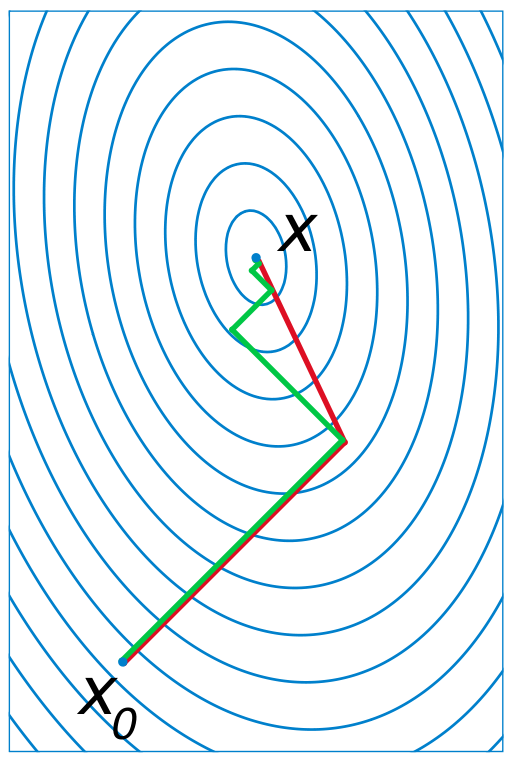
\includegraphics[width=0.5\linewidth]{CG_comparison.png}}
    \caption{Comparison between Conjugate gradient (red) and Gradient descent (green) methods. This is done with the same starting point and an optimal step size for the GD.}
    \label{fig:cg_comp}
\end{figure}

The way we start with the derivation is with the definition of an $A$-matrix inner product for any two vectors
\begin{equation}
    \left( u, v \right)_A = u^\top A v
    \label{eq:cg_constraint}
\end{equation}
and if the product is equal to zero, these vectors are conjugate. Now, we can make a basis of mutually conjugate vectors $\{ p_i \}$, so that we could represent the solution $x'$ of (\ref{eq:lineq}) as a linear combination
\begin{equation}
    x' = \sum_i \alpha_i p_i,
\end{equation}
where
\begin{equation}
    \alpha_i = \frac{\left( p_i, b \right)}{\left( p_i, p_i \right)_A}
\end{equation}

In most cases it is not possible to get the exact result, due to round off error, and one must be content with an approximation of the true result. This means that we do not actually need all conjugate vectors of the basis in order to find a good solution, but we can progressively add more vectors until we are satisfied with the solution.

To show this, we start again with (\ref{eq:lineq}) which is the minimizer (gradient) of a quadratic function
\begin{equation}
    \begin{aligned}
        f(x) &= \frac{1}{2} x^\top A x - x^\top b
        \\
        \nabla f(x) &=  Ax - b
    \end{aligned}
\end{equation}
The goal is to find the minimum, so we define a residual 
\begin{equation}
    r_k = b - Ax_k,
\end{equation}
which measures how close we are to the minimum. And iteratively, the new residual can be computed from the previous
\begin{equation}
    r_{k+1} = r_k - \alpha_k Ap_k,
\end{equation}
where
\begin{equation}
    \alpha_k = \frac{\left( r_k, r_k \right)}{\left( p_k, p_k \right)_A}
\end{equation}
In the Steepest descent method, we use the residuals as search directions, but the improved version that we work with, puts a constraint (\ref{eq:cg_constraint}) on the searches. In order to ensure that the directions are linearly independent, we perform some form of Gram-Schmidt orthogonalization procedure on the residuals where every new $A$-orthogonal vector can be calculated from the previous
\begin{equation}
    p_{k+1} = r_{k+1} + \beta p_k,
\end{equation}
where
\begin{align}
    \beta &= \frac{\left( r_{k+1}, r_{k+1} \right)}{\left( r_k, r_k \right)}
\end{align}
And the new solution can be found by
\begin{equation}
    x_{k+1} = x_k + \alpha_k p_k
\end{equation}
A detailed derivation of CG can be found in [Y. SAAD]. The whole method can be implemented in an algorithm which can be written in pseudocode (Algorithm \ref{alg:cg}) like

\begin{algorithm}
    \caption{Conjugate Gradient}
    \begin{algorithmic}[1]
        \State Initialize  $A, x_0, b$
        \State Initialize $\epsilon$ \Comment{Convergence criteria}
        \State Set $r_0 = b - Ax_0$ \Comment{Initial Condition}
        \State Set $p_0 = r_0$ \Comment{Initial Search Direction}
        \While{$r_{k+1} > \epsilon$}
            \State Set $\alpha_k = \frac{\left( r_k, r_k \right)}{\left( Ap_k, p_k \right)}$
            \State Update $x_{k+1} = x_k + \alpha_k p_k$
            \State Update $r_{k+1} = r_k - \alpha_k Ap_k$
            \State Set $\beta = \frac{\left( r_{k+1}, r_{k+1} \right)}{\left( r_k, r_k \right)}$
            \State Update $p_{k+1} = r_{k+1} + \beta p_k$
        \EndWhile
    \end{algorithmic}
    \label{alg:cg}
    \end{algorithm}

\subsection{Flexible Generalized Minimum Residual}

This method is a variant of the GMRES method with preconditioning. It is called flexible because it can have different preconditioning on each step of the algorithm, whereas in the previous versions it can have only the same preconditioner on each step. It will be easier to understand the whole FGMRES method if we first explain how the preconditioned GMRES works.

The GMRES algorithm is trying to find an approximate solution to (\ref{eq:lineq}) by building a Krylov subspace, which is defined as
\begin{equation}
    \mathcal{K}_n = \mathcal{K}_n (A, r_0) = span \{ r_0, Ar_0, A^2r_0,\hdots, A^{n-1}r_0 \}
\end{equation}
An important property of this subspace is that the vectors are linearly independent, therefore we can use them as a basis to represent our solution. This is done by applying an Arnoldi method, which can find an orthonormal basis in $\mathcal{K}_n$. The process creates a matrix $\bar{H}_m = H_{(m+1)\times m}$. This matrix is used for minimizing the residual $y_m = min(\beta e_1 - \bar{H}_m y)$, which updates the approximation of the solution $x_m = x_0 + Z_my_m$.

As it was written before, this method is robust but slow. So, in order to improve the speed of convergence, we can precondition the original matrix. In FGMRES, we use the right preconditioning
\begin{equation}
    AM^{-1}(Mx) = b,
\end{equation}
where $M$ is a matrix that can be found very easy with another algorithm by solving $Mz = v$. One could use a lot of different methods for preconditioning. They could be not only one-step methods but also iterative techniques like SSOR, ADI, CG, and even GMRES. The detailed derivation of the method can be found in [Y.SAAD], but here we can only show the general idea of the algorithm with a pseudocode (Algorithm \ref{alg:fgmres})

\begin{algorithm}
    \caption{Flexible Generalized Minimum Residual}
    \begin{algorithmic}[1]
        \State Initialize $\epsilon$ \Comment{Convergence criteria}
        \State Initialize  $A, x_0, b$
        \State Initialize $\bar{H}_m$
        \While{$r_m > \epsilon$}
            \State Compute $r_0 = b - Ax_0$
            \State Set $\beta = ||r_0||$
            \State Compute $v_1 = \frac{r_0}{\beta}$
            \For{$j = 1, 2, ..., m$} \Comment{Arnoldi process}
                \State Compute $z_j = M^{-1}_jv_j$ \Comment{Preconditioning (could be different on every step)}
                \State Compute $w = Az_j$
                \For{$i = 1, ..., j$}
                    \State Compute $h_{i,j} = (w, v_i)$
                    \State Compute $w = w - h_{i,j}v_i$
                \EndFor
                \State Set $h_{j+1,j} = ||w||$
                \State Set $v_{j+1} = \frac{w}{h_{j+1,j}}$
            \EndFor
            \State Set $Z_m = [z_1, ..., z_m]$
            \State Compute $y_m = min(\beta e_1 - \bar{H}_m y)$ \Comment{Least square minimization}
            \State Update $x_m = x_0 + Z_my_m$
            \State Update $r_m = b - Ax_m$
            \State Set $x_0 = x_m$
        \EndWhile
    \end{algorithmic}
    \label{alg:fgmres}
    \end{algorithm}